% This is "sig-alternate.tex" V2.1 April 2013
% This file should be compiled with V2.5 of "sig-alternate.cls" May 2012
%
% This example file demonstrates the use of the 'sig-alternate.cls'
% V2.5 LaTeX2e document class file. It is for those submitting
% articles to ACM Conference Proceedings WHO DO NOT WISH TO
% STRICTLY ADHERE TO THE SIGS (PUBS-BOARD-ENDORSED) STYLE.
% The 'sig-alternate.cls' file will produce a similar-looking,
% albeit, 'tighter' paper resulting in, invariably, fewer pages.
%
% ----------------------------------------------------------------------------------------------------------------
% This .tex file (and associated .cls V2.5) produces:
%       1) The Permission Statement
%       2) The Conference (location) Info information
%       3) The Copyright Line with ACM data
%       4) NO page numbers
%
% as against the acm_proc_article-sp.cls file which
% DOES NOT produce 1) thru' 3) above.
%
% Using 'sig-alternate.cls' you have control, however, from within
% the source .tex file, over both the CopyrightYear
% (defaulted to 200X) and the ACM Copyright Data
% (defaulted to X-XXXXX-XX-X/XX/XX).
% e.g.
% \CopyrightYear{2007} will cause 2007 to appear in the copyright line.
% \crdata{0-12345-67-8/90/12} will cause 0-12345-67-8/90/12 to appear in the copyright line.
%
% ---------------------------------------------------------------------------------------------------------------
% This .tex source is an example which *does* use
% the .bib file (from which the .bbl file % is produced).
% REMEMBER HOWEVER: After having produced the .bbl file,
% and prior to final submission, you *NEED* to 'insert'
% your .bbl file into your source .tex file so as to provide
% ONE 'self-contained' source file.
%
% ================= IF YOU HAVE QUESTIONS =======================
% Questions regarding the SIGS styles, SIGS policies and
% procedures, Conferences etc. should be sent to
% Adrienne Griscti (griscti@acm.org)
%
% Technical questions _only_ to
% Gerald Murray (murray@hq.acm.org)
% ===============================================================
%
% For tracking purposes - this is V2.0 - May 2012

\documentclass{sig-alternate-05-2015}
\usepackage{color}

\begin{document}

% Copyright
\setcopyright{acmcopyright}
%\setcopyright{acmlicensed}
%\setcopyright{rightsretained}
%\setcopyright{usgov}
%\setcopyright{usgovmixed}
%\setcopyright{cagov}
%\setcopyright{cagovmixed}


% DOI
\doi{10.475/123_4} 

% ISBN
\isbn{123-4567-24-567/08/06}

%Conference
\conferenceinfo{PLDI '13}{June 16--19, 2013, Seattle, WA, USA}

\acmPrice{\$15.00}

%
% --- Author Metadata here ---
\conferenceinfo{WOODSTOCK}{'97 El Paso, Texas USA}
%\CopyrightYear{2007} % Allows default copyright year (20XX) to be over-ridden - IF NEED BE.
%\crdata{0-12345-67-8/90/01}  % Allows default copyright data (0-89791-88-6/97/05) to be over-ridden - IF NEED BE.
% --- End of Author Metadata ---

\title{YouUnderstood.me? Personalized Readability-based Retrieval of Online Materials for Students and Educators}

%
% You need the command \numberofauthors to handle the 'placement
% and alignment' of the authors beneath the title.
%
% For aesthetic reasons, we recommend 'three authors at a time'
% i.e. three 'name/affiliation blocks' be placed beneath the title.
%
% NOTE: You are NOT restricted in how many 'rows' of
% "name/affiliations" may appear. We just ask that you restrict
% the number of 'columns' to three.
%
% Because of the available 'opening page real-estate'
% we ask you to refrain from putting more than six authors
% (two rows with three columns) beneath the article title.
% More than six makes the first-page appear very cluttered indeed.
%
% Use the \alignauthor commands to handle the names
% and affiliations for an 'aesthetic maximum' of six authors.
% Add names, affiliations, addresses for
% the seventh etc. author(s) as the argument for the
% \additionalauthors command.
% These 'additional authors' will be output/set for you
% without further effort on your part as the last section in
% the body of your article BEFORE References or any Appendices.

\numberofauthors{2} %  in this sample file, there are a *total*
% of EIGHT authors. SIX appear on the 'first-page' (for formatting
% reasons) and the remaining two appear in the \additionalauthors section.
%
\author{
% You can go ahead and credit any number of authors here,
% e.g. one 'row of three' or two rows (consisting of one row of three
% and a second row of one, two or three).
%
% The command \alignauthor (no curly braces needed) should
% precede each author name, affiliation/snail-mail address and
% e-mail address. Additionally, tag each line of
% affiliation/address with \affaddr, and tag the
% e-mail address with \email.
%
% 1st. author
\alignauthor
Ion Madrazo\\
       \affaddr{Computer Science Department}\\
       \affaddr{Boise State University}\\
       \affaddr{Boise, Idaho, USA}\\
       \email{ionmadrazo@boisestate.edu}
% 2nd. author
\alignauthor
Maria Soledad Pera\\
       \affaddr{Computer Science Department}\\
       \affaddr{Boise State University}\\
       \affaddr{Boise, Idaho, USA}\\
       \email{solepera@boisestate.edu}
}
% There's nothing stopping you putting the seventh, eighth, etc.
% author on the opening page (as the 'third row') but we ask,
% for aesthetic reasons that you place these 'additional authors'
% in the \additional authors block, viz.

\date{30 July 1999}
% Just remember to make sure that the TOTAL number of authors
% is the number that will appear on the first page PLUS the
% number that will appear in the \additionalauthors section.

\maketitle
\begin{abstract}
K-12 students and educators make use of online resources to satisfy
their academic information needs on a daily basis. Unfortunately, they
are forced to spend large amounts of time seeking for adequate
materials. For students, retrieving materials that are outside their
comprehension level can be discouraging. For educators, finding
materials for curriculum development that suit their students'
individual reading abilities can also be challenging.  We present
\textit{YouUnderstood.me}, a web application that makes use of
information retrieval, natural language processing, and machine
learning to provide an enhanced web search environment that promotes
the synergy between students and educators and helps them locate
materials that match the reading abilities of individual students.
% to help both students and educators in the process of seeking materials that fit the reading skills of each individual student.
\textit{YouUnderstood.me} offers: (1) a search interface that combines
a search module, a search intent module, and a readability-based
filtering module, which leads to the fast retrieval of documents from
different sources, (2) a tracking module that keeps records of
students' feedback on retrieved results, in terms of degrees of
comprehension accomplished, which in turn informs educators of the
change in readability levels of their respective students over time,
and (3) a readability analysis module that enables educators to
estimate the reading level of snippets of texts. The combination of the described modules
make \textit{YouUnderstood.me}, to the best of our knowledge, the
first tool specifically designed for educational environments that
simultaneously aids both teachers and students dealing with personalized online searches.
\end{abstract}


%
% The code below should be generated by the tool at
% http://dl.acm.org/ccs.cfm
% Please copy and paste the code instead of the example below. 
%



\begin{CCSXML}
<ccs2012>
<concept>
<concept_id>10002951.10003260.10003261.10003271</concept_id>
<concept_desc>Information systems~Personalization</concept_desc>
<concept_significance>500</concept_significance>
</concept>
<concept>
<concept_id>10002951.10003317.10003331.10003336</concept_id>
<concept_desc>Information systems~Search interfaces</concept_desc>
<concept_significance>500</concept_significance>
</concept>
<concept>
<concept_id>10003456.10010927.10010930.10010931</concept_id>
<concept_desc>Social and professional topics~Children</concept_desc>
<concept_significance>500</concept_significance>
</concept>
</ccs2012>
\end{CCSXML}

\ccsdesc[500]{Information systems~Personalization}
\ccsdesc[500]{Information systems~Search interfaces}
%\ccsdesc[500]{Applied computing~Interactive learning environments}
%\ccsdesc[500]{Applied computing~Learning management systems}
\ccsdesc[500]{Social and professional topics~Children}



%
% End generated code
%

%
%  Use this command to print the description
%
\printccsdesc

% We no longer use \terms command
%\terms{Theory}

\keywords{Search interfaces; Filtering; Readability; Educational tools}


\begin{figure*}[ht]
 \centering
  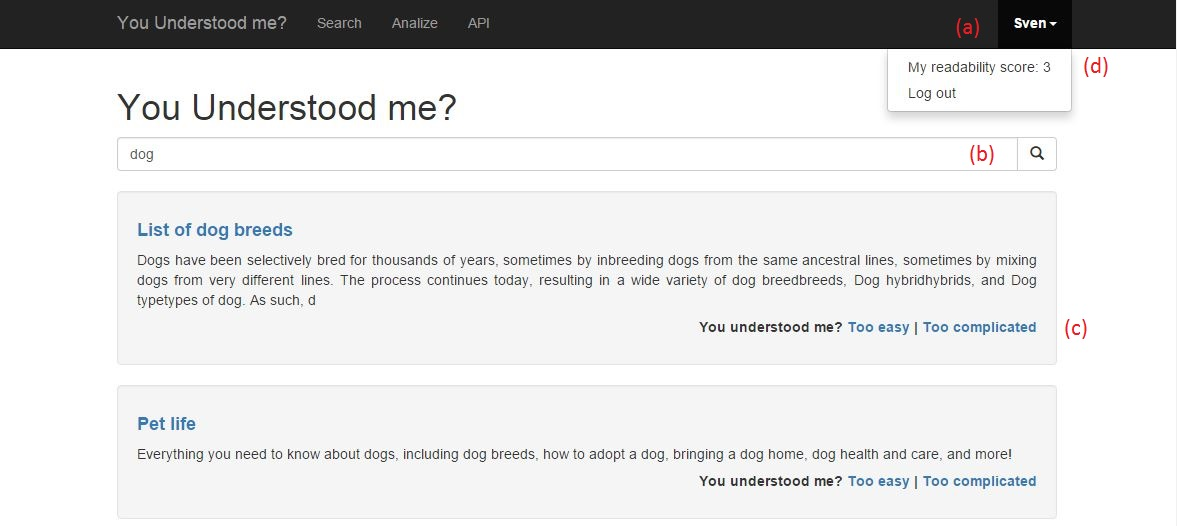
\includegraphics[width=1\textwidth]{creatingFigures/Capture20}
 \caption{Screenshot of \textit{YouUnderstood.me}'s search interface for students}
 \label{fig:studentSearch}
 \end{figure*}



\begin{figure*}[ht]
 \centering
  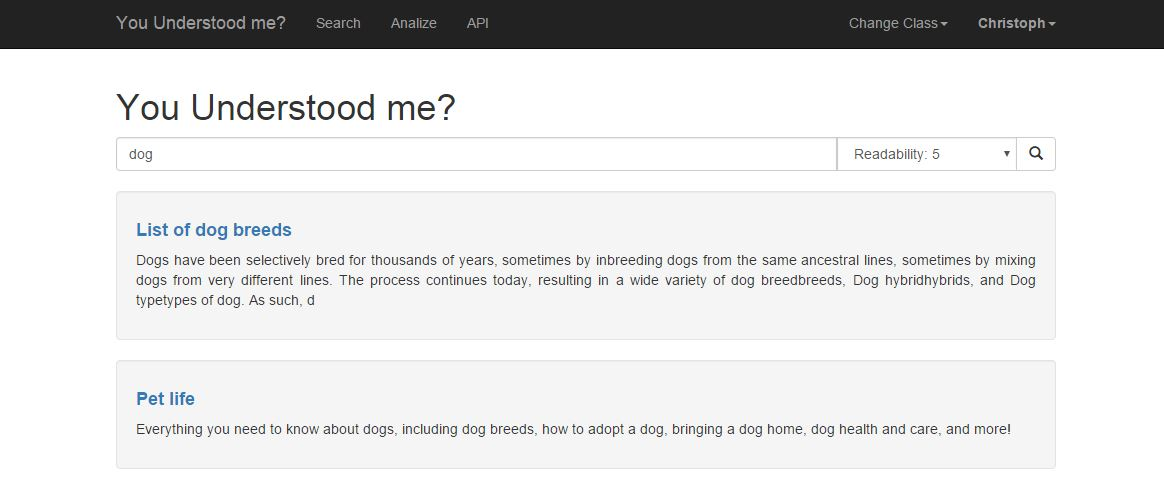
\includegraphics[width=1\textwidth]{creatingFigures/Capture18}
 \caption{Screenshot of \textit{YouUnderstood.me}'s search interface for educators}
  \label{fig:educatorSearch}
 \end{figure*}




\section{Introduction}
\noindent
The use of Web technologies is increasingly becoming a relevant aspect for children education, both because it enhances the class environment and introduces children, from early stages of their lives, into today's information society \cite{sadaf2012exploring}. K-12\footnote{K-12 refers to the publicly-supported school grades prior to college in the education systems from United States of America, Canada and other countries.} students use the internet on a daily basis to locate materials that can help them with different academic tasks, from finding information for a class presentation to discovering the meaning of a new word. For this purpose, they often turn to search engines and online catalogs to retrieve materials that can satisfy their information needs, including news articles, books, or term definitions. However, even if search engines are successful in terms of retrieving relevant resources that are of interest to a general audience, they can be less so when used by niche users \cite{wang2013personalized}, such as K-12 students. Unlike average users, K-12 students have varied  reading abilities, a fact that is usually overlooked by popular search engines. As a result, students can often get discouraged when they try to read retrieved contents that are outside their comprehension level, whether being too easy or too difficult  for them to understand. Therefore, providing K-12 students with tools they can apply to seek for adequate materials they can actually understand is imperative.

%Reading is an important skill in the academic environment, a skill that can have a high impact for a student's educational opportunities and their career \cite{robinson2000issues}. However, students can get discouraged to read, when the texts provided are outside of their comprehension level, whether being too easy to read  or too difficult for them.


Within the academic environment, students are not the only ones facing the problem of locating adequate reading materials that simultaneously match information needs and reading abilities. Educators also face several challenges when looking for materials for their classes, which translates into unnecessary time spent online to accomplish this goal. For example, even in a same grade class, students' reading skills can differ significantly, so not all of them should be given the same texts. As a result, a fair amount of personalization is required, which educators are expected to handle in a daily basis. Unfortunately, given the high number of students in each class, this task can become impossible to tackle. 


%Due to the mentioned fact, instructors spend a significant amount of their time seeking adequate materials for their students, a time that could be reduced with the help of an specialized application.\\

\textit{YouUnderstood.me} is a web application designed to help  both instructors and students in the process of finding online reading materials. The application is centered on the use of readability formulas that together with a search engine and a search intent module make the task of looking for leveled reading materials effective and efficient. By requiring students to log in prior to conducting searches \textit{YouUnderstood.me} can keep track of the feedback they give about the degree of understanding of the read (retrieved) resources (too easy/OK/too complicated). This enables the application to make predictions regarding the reading abilities of each student, which can be used by both students and educators for speeding-up the process of identifying adequate materials. Furthermore, the application integrates a search interface that allows both stakeholders to seek materials filtered by readability levels from: (i) commercial search engines, such as Google, (ii) public data sources, such as Wikipedia and (iii) local resources, such schools' library catalogs. Furthermore, the student search interface also offers a search intent module,
which transform student-formulated queries on-the-fly into queries that can lead to the retrieval of relevant resources. 

%, AR\footnote{http://www.acceleratelearning.com} or Lexile\footnote{http://lexile.com} 

Besides the search interface, instructors also have access to an analysis page, where they can submit texts and estimate their readability scores, based on a wide range of readability formulas provided within the application. This module, together with the track of readability scores of students, helps teachers make sure the reading materials they select are adequate for the respective class or an individual student.

The novelty of \textit{YouUnderstood.me} lays on how its different submodules are combined in order to create an enhanced, personalized, search environment that promotes the synergy between students and teachers to help them locate materials that match the reading abilities of each student.
% an application that becomes helpful in an academic environment.
To the best of our knowledge, \textit{YouUnderstood.me} is the first application that tackles the issue of reading material retrieval as a whole. Starting from the assessment of an individual student's reading ability, and ending with the retrieval of adequate materials, all modules of \textit{YouUnderstood.me} work in cooperation to improve the way in which online reading materials are located.

 
\section{YouUnderstood.me}

%Whether when a student is searching information for completing an assignment or an educator uses the application for finding material for his course, a text's complexity needs to be determined in order to evaluate if the material fits the needs of readability level.\\
\noindent
Regardless of the stakeholder or the task that needs to be performed, \textit{YouUnderstood.me}
takes advantage of readability assessment formulas for estimating the level of difficulty of a reading material. Different approaches have been followed in the literature for determining a text's complexity or readability. Most approaches, focus their work in determining the readability of text snippets. Those systems vary from very simple ones \cite{flesch1948new}, which make use of shallow features, such as the average number of words per sentence or the average length of terms, to more complex ones \cite{dell2011read,franccois2012ai,gonzalez2014simple}, which are mostly based on supervised learning techniques and features extracted using Natural Language Processing. Those tools, however, have shown to be of little use in contexts where the text of the corresponding material has reduced accessibility, both because the text is not publicly accessible or because it shows a structure not as simple to tackle. Consequently, different works have been done in more specialized contexts such as book \cite{denning2015readability,pera2014automating} or web page retrieval \cite{lau2006bilingual}, where the systems presented take advantage of domain dependent features.


\textit{YouUnderstood.me} integrates a readability assessment module than can make use of different metrics and resources simultaneously, aiming to handle a more diverse amount of reading materials. The methods with which \textit{YouUnderstood.me} can predict text complexity are the following:

\begin{itemize}
\item \textbf{External metrics.} \textit{YouUnderstood.me} is compatible with the most popular readability metrics among the American education system, such as AR\footnote{www.acceleratelearning.com} or Lexile\footnote{www.lexile.com}. The aforementioned metrics are widely used for measuring the readability of books from children curricula. This permits \textit{YouUnderstood.me} retrieve books, which would be difficult to handle otherwise, because of the inability to get access to the contents of copyrighted material.
\item \textbf{Traditional formulas.} Historically used by teachers for manually determining the readability level of a reading material, traditional formulas such as Flesh \cite{flesch1948new}, Fog\cite{gunning1952technique} and Flesh-Kincaid \cite{flesch1948new}, are also supported by \textit{YouUnderstood.me}. 
\item \textbf{MRAS.} MRAS (Multilingual Readability assessment system)\cite{imadrazo2016readability} is a state-of-the-art readability assessment system, which is capable of detecting the input language of a text on-the-fly and providing the corresponding readability score. MRAS is based on a supervised learning paradigm, that makes use of more than a hundred features for readability prediction. 

%The features are extracted using Natural Language Processing tools, such as a tokenizer, a part of speech tagger and different semantic analyzers. Those features, are used to train a model that will later be used for predicting the readability score for new materials.


\end{itemize}

Stakeholders of \textit{YouUnderstood.me} can benefit from the aforementioned readability scores in different ways. \textbf{Students} can make use of a \textbf{search engine} (as illustrated in Figure \ref{fig:studentSearch}) which provides several features that are aimed at helping them in the process of seeking adequate reading materials. In order to use it, the student needs to be logged in (a), which permits the application personalize his search experience.

Each query a student formulates is first treated with an ad-hoc search intent module that is capable of solving issues that usually arise while processing children queries and that can lead children to retrieve poor results, such as misspelling, children popular culture terms or queries that are too long. Processed queries are submitted to a search engine. Currently two methods of search are implemented: one that makes use of the Google Search API and another one based on the Apache Lucene\footnote{lucene.apache.org/} framework.


Documents retrieved by the search engine are analyzed and filtered based on the readability requirements of each individual student. The documents can be both dynamically or statically analyzed, depending on their source and the search tool used. For example, documents are analyzed on the fly when using Google. This requires the readability prediction to be fast, forcing the application to use a lightweight readability formula such as Flesch or FOG. However, when using Lucene, documents can be previously analyzed (offline), enabling the use of more complex readability prediction tools, such as MRAS.

Once the student has read the chosen material, he can provide feedback on it (c), helping the system to improve the filtering for future searches. This feedback is recorded based on the option (among the three provided) selected by the student, which reflect whether the material was too easy, OK, or too complicated to understand. This information is provided to \textit{YouUnderstood.me}'s tracking module to adjust future predictions about individual users' reading skills.

The \textbf{tracking module} is currently based on a trivial method of approximation which simply increases each student's readability level every time he finds a recommended reading material too easy, and decreases it, every time he finds it too complicated. However, we are aware that more precise methods exist and plan to implement them in the near future. An updated prediction of the system regarding each student can be seen on the profile menu (d), allowing each student to keep track of the progress he is making.
\begin{figure*}[ht]
 \centering
  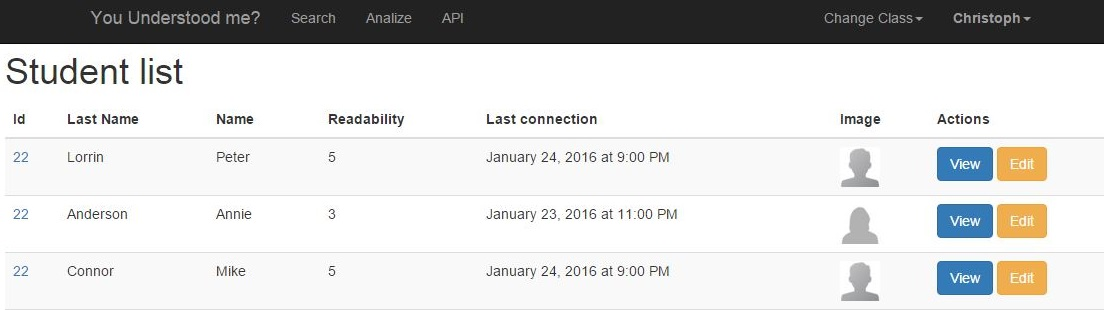
\includegraphics[width=1\textwidth]{creatingFigures/Capture19}
 \caption{Screenshot of student list for educator}
  \label{fig:studentList}
 \end{figure*}

\textbf{Educators} can also make use of the \textbf{search interface}, which is adapted to their use (see Figure \ref{fig:educatorSearch}). The educator view of the search engine enables the user to choose the readability level he wants. Moreover, the search engine no longer makes use of the search intent module, given that teachers are able to formulate queries that reflect their intended information needs, and thus adding this extra layer of filtering would only hinder their work. Furthermore, the readability level for filtering the reading materials is no longer decided by the system, giving the instructor the option for choosing the level of challenge he wants for his students. The feedback options are no longer available either, since there is no point in evaluating the educator's reading ability.

\textbf{Educators} can also use the material analysis tool (see Figure \ref{fig:analysispage}) that allows them to analyze snippets of text. This module offers a choice of readability formulas to be considered for analysis purposes, among the formulas that have already been mentioned.


\begin{figure}[h!]
 \centering
  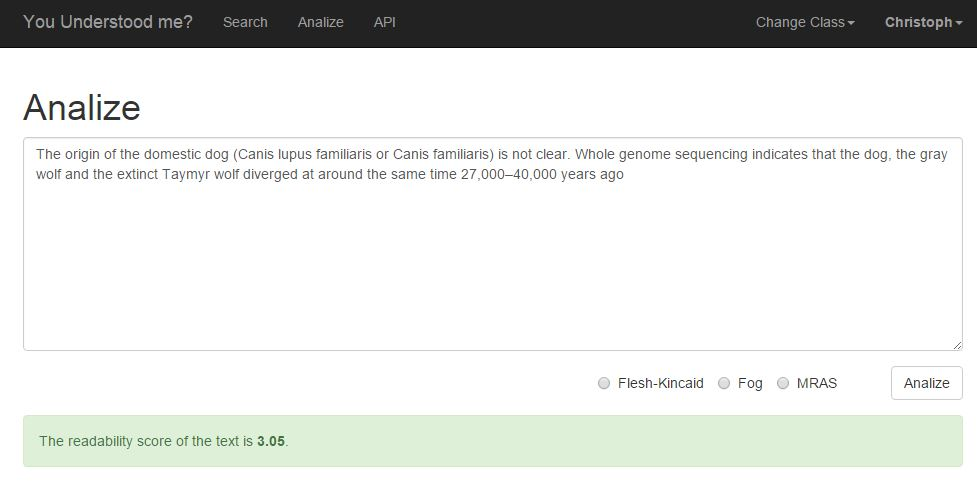
\includegraphics[width=0.45\textwidth]{creatingFigures/Capture22}
 \caption{Screenshot of the analysis page of \textit{YouUndestood.me}}
 \label{fig:analysispage}
 \end{figure}
 
 
 
Finally, a student tracking tool is provided for educators (Figure \ref{fig:studentList}). This module provides a fast way to discover either the individual or overall reading skills of students in a given class. The educator can view a prediction for individual students' reading skills or go deeper and view the feedback that the student gave for each of the reading materials.


%The document analyzer is the center of the the application
%It is used for both analysis tool and material searcher
%

%Where does it work, catalogs, internet, enciclopedias
%How does it work, search filtering?

\begin{comment}
\section{User Experience}

\begin{itemize}
\item \textbf{Analyzing materials.} An analysis page is provided to instructors, so that they can make use of the readability assessment algorithm \cite{imadrazo2016readability} with materials from outside the application. This page provides an input form where the instructor can submit the material, and receive the corresponding readability level prediction.

\item \textbf{Looking for new materials.} A material search page is provided so that the user can submit queries that capture their information needs. The user can select a certain readability level he wants to look for, of leave it blank, letting the application choose the best level for the logged user. Furthermore, the material source can be selected, depending on the user needs. In the case of students, they can select a material for reading and provide feedback on it. This feedback will be used for tracking purposes.

\item \textbf{Tracking students.} The educator can see a table with data about all his students, where the number of materials read and the readability score for each student are provided. The instructor can go deeper if needed, and see each of the materials each students has read and the individual readability scores for each material, as well as, the feedback given by the student. The data is also presented in a summarized way, so that the educator can see the average, maximum and minimum reading skills of the students in class.

\end{itemize}

\end{comment}

\section{Conclusion and Future work}



\noindent
We have introduced \textit{YouUnderstood.me}, a web application that simplifies the task of seeking for adequate online resources in terms of readability levels, within an academic environment. \textit{YouUnderstood.me} adopts a modular design, which facilitates the task of simultaneously integrating different readability prediction strategies, material sources
%, as well as ...
, making it extensible and versatile. It provides an environment tailored to different types of users: students and educators. Students can benefit from a personalized search interface which combines a search intent module and retrieved results filtered by the corresponding readability level %ty filtered search engine that personalizes results towards 
of each individual student. At the same time, educators can take advantage of three different modules, i.e., a search interface, which aids educators in locating materials tailored to individual students, a readability analysis tool, which can help them in writing of tests or directions for homework assignments and ensuring that their students can understand them, and a student tracking system,  which speeds up the process of locating reading materials suitable to the abilities of each student in class. All the mentioned modules work in cooperation to create, to the best of our knowledge, the first educational tool that tackles the reading material seeking problem as a whole.

On the future, we would like to focus our work on enhancing the synergy between educators and students even more. We would like to give educators a way to validate students' queries, so that students can know which mistakes were included in their queries. This way, students would progressively improve their query formulation skills. We would also want to enhance \textit{YouUnderstood.me} to encourage collaborative searches among students and educators.  All these features would lead \textit{YouUnderstood.me} to be an even more versatile tool, a tool that would truly make students and educators understand each other.







%TODO FUTURE WORK
%UUM is equipped with modules that provide students with online materials that match their reading abilities. 

%Furthermore, UUM includes a search intent module that facilitates the task of creating queries on-the-fly that can lead to the retrieval of suitable resources.

%UUM keeps track of student feedback (in terms of the readability level of the retrieved resources) 

%Educators can see the readability levels of each of their students, which speeds up the process of locating reading materials suitable to the abilities of each student in the class

%Educators can also detect the readability level of text snippets, which can help them in the writing of tests or directions for homework assigments and thus ensure that their students can understand them.

%UUM adopts a modular design, which facilitates the task of simultaneously integrating different text-prediction strategies.

%UUM will be extended over time, so that it can be applicable to languages other than English. More importantly, it will grow to provide a search enviroment that students and educators can take advantage of

%more future work is needed
%wrap up is the last thing reviewers will remember, so it needs to have a big impact.






\bibliography{bibliography}{}
\bibliographystyle{abbrv}
%\nocite{*}
\end{document}
